\documentclass[a4paper]{article}

%%% packages %%%%%%%%%%%%%%%%%%%%%%%%%%%%%%%%%%%%%%%%%%%%%%%%%%%%%%%%%%%%%%%%%
\usepackage{graphicx}
\usepackage{amsmath,amssymb}
\usepackage{alltt}
\usepackage{natbib} % please use \citep and \citet instead of \cite

\usepackage{hyperref}
\usepackage{xcolor}
\definecolor{dark-red}{rgb}{0.4,0.15,0.15}
\definecolor{dark-blue}{rgb}{0.15,0.15,0.8}
\definecolor{medium-blue}{rgb}{0,0,0.5}
\hypersetup{
    colorlinks, linkcolor={dark-red},
    citecolor={dark-blue}, urlcolor={medium-blue}
}

\graphicspath{{./figs/}}
\DeclareGraphicsExtensions{.pdf}

\setlength{\parindent}{0mm}

\usepackage{fancyhdr}

%%% %%%%%%%%%%%%%%%%%%%%%%%%%%%%%%%%%%%%%%%%%%%%%%%%%%%%%%%%%%%%%%%%%%%%%%%%%

\makeatletter
\newcommand{\seminar}{Seminar Cyber-Physical Systems (WS 2019/20)}
\title{Your Title}\let\Title\@title
\newcommand{\sTitle}{YourShortTitle}
\newcommand{\AuthorName}{YourFirstname YourLastname}
\author{\AuthorName\\
  \href{mailto:xx.yy@student.uni-luebeck.de}{xx.yy@student.uni-luebeck.de}\\
  \small \seminar\\
  \small Service Robotics Group\\
  \small Institute of Computer Engineering, University of L\"ubeck\\
}\let\Author\@author
\makeatother

\pagestyle{fancy}
\renewcommand{\footrulewidth}{0.4pt}
\lfoot{\seminar}
\cfoot{}
\rfoot{\thepage}
\lhead{\AuthorName}
\rhead{\sTitle}

%%% %%%%%%%%%%%%%%%%%%%%%%%%%%%%%%%%%%%%%%%%%%%%%%%%%%%%%%%%%%%%%%%%%%%%%%%%%

\begin{document}
\maketitle

\begin{abstract}
  \noindent%
  Abstract starts here
\end{abstract}


\section{Introduction}

Swarm robotics~\citep{brambilla13} bla bla bla.
\citet{hamann18} describes bla bla bla
see Sec.~\ref{sec:results}


\section{Results}
\label{sec:results}

see Fig.~\ref{fig:image}

\begin{figure}[t]
  \centering
  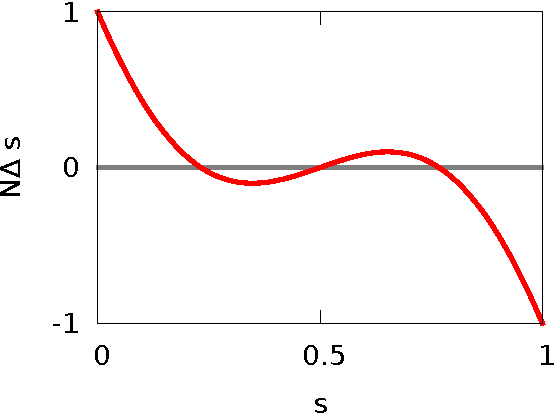
\includegraphics[angle=0,width=0.4\textwidth]{./figs/swarmDelta}
  \caption{\label{fig:image}bla.}
\end{figure}



\section{Conclusion}


\footnotesize
\bibliographystyle{plainnat}
\bibliography{./main}

\end{document}
